\chapter{Traffic Science}

\section{Introduction}

\paragraph{Terminology}

In the rest of the document I will refer to \textit{transit} or \textit{flow} to indicate a group of traveling vehicles.
The word \textit{traffic} will be used only indicate the phenomenon of high density flows where there is the perception of being slowed down.
The word \textit{jam} will indicate strictly a deadlock traffic event.

\paragraph{Vehicles}

This is a umbrella term for referring to any kind of entity which travels along a network.
Vehicles \textbf{can} have an \textit{origin} and a \textit{destination}: for example, private motor vehicles are usually driven in order to go from a \textit{point-of-interest} A to a point point-of-interest B.
An interesting exception are those public transit vehicles serving on a \textit{circle line} like the M3 City Circle Line of Copenhagen, and in general vehicles offering public transit logically have more than one destination while carrying out a trip.
Vehicles attempt to follow a \textit{desired path}, which is influenced by various factors: network knowledge, habits, transit regulations and so on.
This path can diverge from the \textit{actual path} they end up following for various reasons: accidents, infrastructure works, events and maybe illegal parking.
A notable exception are fixed route vehicles (such as public transit) and in particular track-constrained vehicles (such as trams and trains).
In both cases, the whole journey is not required to be completed: a vehicle can override its route because of change of heart (the case of private vehicles), rescheduling (the case of public transit) or else.
Depending on the goal of a simulation, the flow can be restricted to a small set of vehicle types, but in the real world, the vehicle flow can be heterogeneous: cars, trolleybuses, trams, emergency vehicles, trucks, bicycles, motorbikes and so on. Each vehicle has different physical properties and different allowances.
Vehicles allowance rules can be defined by diving the flow with respect to origin/destination, vehicle type (cars \textit{mustn't} ride in bike lanes), local regulations (in some cities, taxis \textit{may} use public transit lanes), vehicle properties (\textit{only} motor vehicles able to reach at least 60 km/h can drive on the motorway) or even driver properties (\textit{limited traffic zones} are open only for residents).
This partitioning activity is a form of transit regulation and characterizing vehicles by their properties rather than transparent objects helps (TODO: CITAZIONE) in managing their transit, resolving path conflicts and also enhancing the quality of life of residents (a bypass \textit{should} cut a significant amount of transit vehicles in city centers).

\paragraph{Infrastructure}

The road network can be represented with a \textbf{directed multi-graph} of intersections and roads. Each road has one or more lanes, a maximum speed and vehicles allowances dictating which kind of vehicles are allowed to flow through it. While more simplistic models use undirected graph with labelled edges to represent lanes and one/two-way traffic, it should be noted that a simple directed graph wouldn't be sufficient as in real-world road networks the may be more different links between an intersection. While some network slices could be represented with a single edge, there are more complex situations as in figure \ref{fig:multigraph-is-better-than-nothing} (a slice of Viale Zara, Milan, Italy) in which two big intersections are linked with two main one-way three-lane roads, two side one-way one-lane roads ("controviali") and two dedicated links for tramway vehicles. These roads are physically separated with median strips and each link may allow for different turns within the intersections. Of course, the implementation model can be optimized for performance, but the logical model should remain a multi-graph because it better represents the features of the road network.

\paragraph{Traffic}

\textbf{Traffic} can be defined as a flow of vehicles on a network with peaks of density in some locations in which the average speed of those vehicles is significantly lower than the average of the entire network.
Mathematically speaking, \textbf{traffic} emerges when many vehicles need or want to transit through a shared path which hasn't enough capacity for handling this high number of users.
Urban planning authorities have since then taken this hint quite literally, adding lanes year-by-year, but in the end the only result was an increase in the number of road vehicles with unchanged transit density or, even worse, with higher travel times \cite{Speck2018}.
In this context, \textbf{traffic science} comes in help: it seeks to understand the causes of traffic as a social \textit{phenomenon} modeling demand and analyzing flaws and strengths of infrastructure.

In the following sections I'll explain and analyze the impact of some strategies for transit regulation and traffic reduction. I'll introduce the concepts of demand modeling. Finally I'll explain the main assumptions for the present simulation and present the scenarios being used.

\section{Transit Regulation}

All the strategies presented in this section involve the usage of infrastructure artifacts in order to optimize transit. The first group aims to manage excessive flows by organizing them into different streams by origin, destination or mean of transportation and modifying the road infrastructure. The second aims to reduce route conflicts and optimize the usage of intersections. None of those is able to "fix" traffic, there are no silver bullets. This section is intended to introduce the reader to the context of transit regulation.

\subsection{Managing high flows}

\paragraph{Just one more lane}

What happens when among all the route that can be possibly be followed there is one which is faster and more convenient? Different streams are going to merge into a single huge flow which is slower than the other ones. A reasonable but ineffective action is to increase the number of lanes \ref{fig:atlanta-georgia-freeway}, but that adds only capacity to the system. It temporally fluidify traffic until other vehicles arrive into the system because it has become more convenient than their current route, and eventually traffic reemerges.

\paragraph{Bypasses, freeways, motorways}

Freeways and motorways are an example of \textit{specialized roads} which can be used to segregate the flows of vehicles needing to travel long distances from the local/regional transit. Those are generally built far from urban areas and those are what prevented urban planners from extending local roads into ten-lanes wide monsters. A further example of specialized road are bypasses, which are used to cut travel times and reduce the number of vehicles that go through the city center, but can also be used in combination with motorways. For example, there is a project to build a bypass in the Bologna's motorway node to split the flow on the basis of whether those vehicles are going to Bologna or need to reach other destinations like Firenze and Ancona. Specialized roads are generally effective in reducing travel times and represent the more convenient way for traveling mid/long distances, however they require extensive land usage and are subject to increased demand. As they essentially only add capacity to the system, it's only a matter of time before vehicle density reaches jamming levels.

\paragraph{Transit zones}

The urban area can be divided into \textit{zones} in which some vehicles can or cannot enter with various kind of rules. \textit{Restricted traffic zones} (\textbf{ZTL}) are effectively used in city centers to block the entrance of non-resident vehicles and reduce the number of vehicles in the area.
\textit{Controlled access zones} (\textbf{CAS}) are similar but only require the payment of a toll in order to enter in the zone. An infamous example is the Area C of the city of Milan, where in order to enter it, the driver needs to buy a ticket (but some vehicles are exempts). Usually, the toll is used as a deterrent for persuading drivers to avoid central areas.
Finally, in \textit{Low emission zones} (\textbf{LEZ}) the only vehicles which entrance is forbidden are the ones exceeding pollution limits (e.g. by Europe emission standards). This measure is effective only in those societies where electric vehicles (EVs) make up a small percentage of registered vehicles, because otherwise a large number of vehicles would not be affected by this regulation.

%% Restricted traffic zones (ZTL)
%% Controlled access zones
%% Low emission zones

\paragraph{Dedicated lanes}

%% Bike lanes
%% Public transit lanes

\paragraph{One-way roads}

\subsection{Managing conflicts}

%% Normal intersections
%% Roundabouts
%% Traffic lights
%%% Green-way
%%% Public service synchronization ("asservimento semaforico")

\section{Demand models}

%% When: Rush-hour models
%% Where-to-where: Origin/Destination models

\section{Assumptions}

% Only cars
% Syntetic data
% Baseline traffic lights are using green-wave mode of operation
% Syntetic queues

\section{Scenarios}

% Breda
% Celoria

\section{Figures}

\begin{figure}[h]
    \centering
    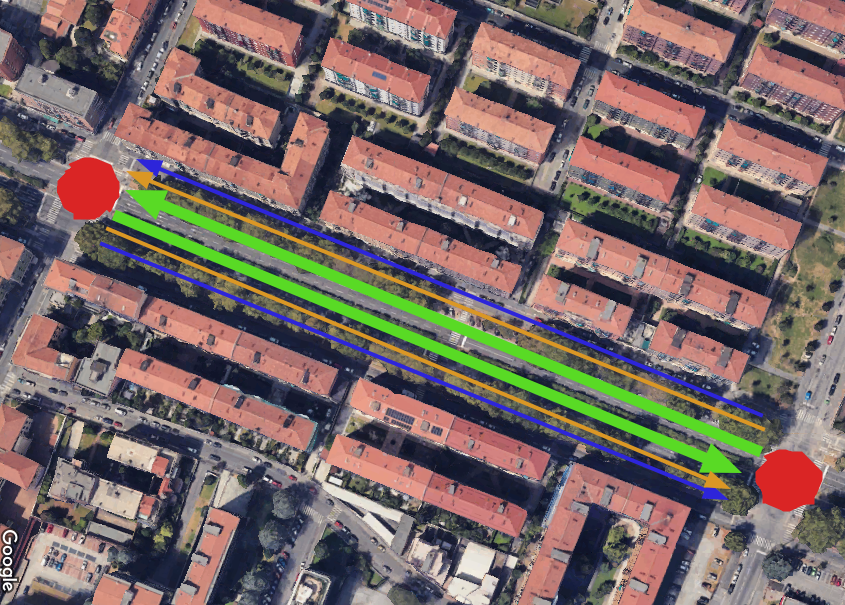
\includegraphics[width=0.75\linewidth]{figures/multigraph-is-better-than-nothing.png}
    \caption{A complex intersection pair which is connected with more different roads (Viale Zara. Milan. Italy). In \textit{green} the main lanes, in \textit{blue} the side lanes, in \textit{orange} the tramway.}
    \label{fig:multigraph-is-better-than-nothing}
\end{figure}

\begin{figure}[h]
    \centering
    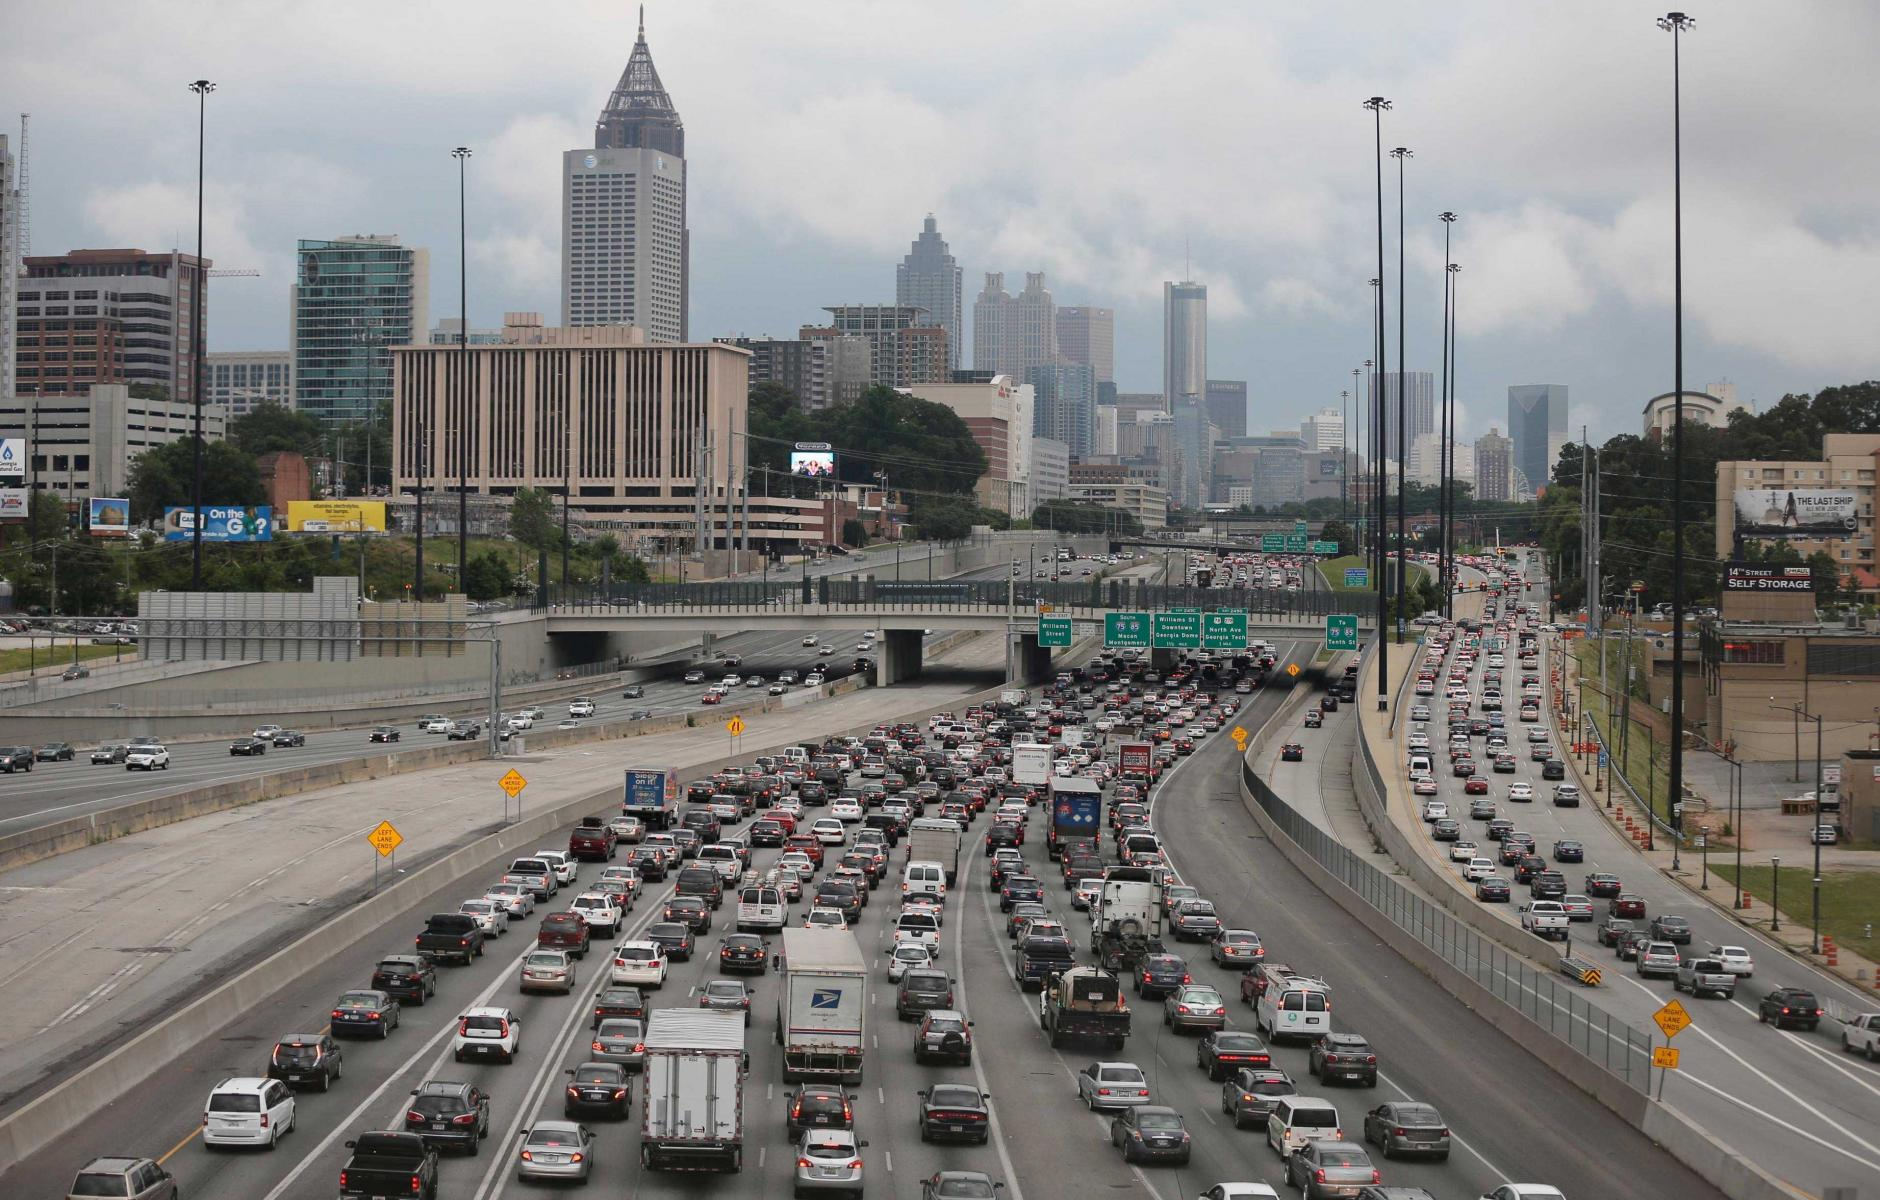
\includegraphics[width=0.75\linewidth]{figures/atlanta-georgia-freeway.jpg}
    \caption{A view of Atlanta Freeway, Georgia}
    \label{fig:atlanta-georgia-freeway}
\end{figure}

\begin{figure}[h]
    \centering
    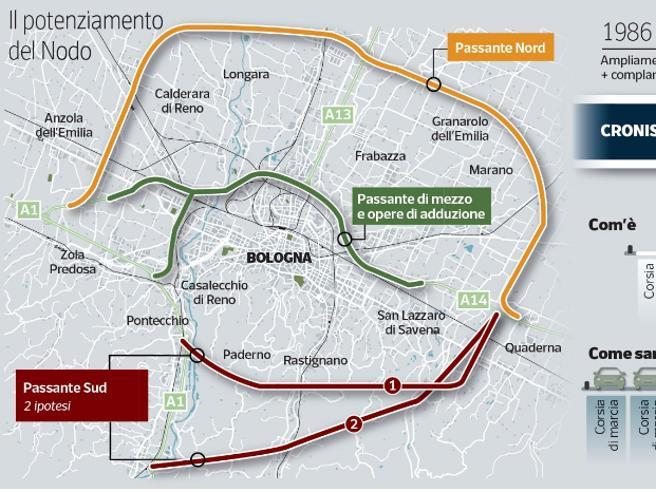
\includegraphics[width=0.75\linewidth]{figures/bologna-bypass.jpg}
    \caption{Highlight of alternatives for the Bologna node bypass}
    \label{fig:bologna-bypass}
\end{figure}
